\documentclass{article}
\usepackage[utf8]{inputenc}
\usepackage{natbib}
\usepackage{graphicx}

\title{Algoritimos e Estrutura de Dados}
\author{Felipe Muniz de Araujo}
\date{Novembro 2019}

\begin{document}

\maketitle

\section{Introdução}
Os algoritmos são instruções que visam a solução de um problema, um exemplo clássico é a receita de bolo. Esta disciplina apresenta conceitos sobre algoritmos, estruturas de dados e complexidade.\citep{site}

\begin{figure}[h!]
    \centering
    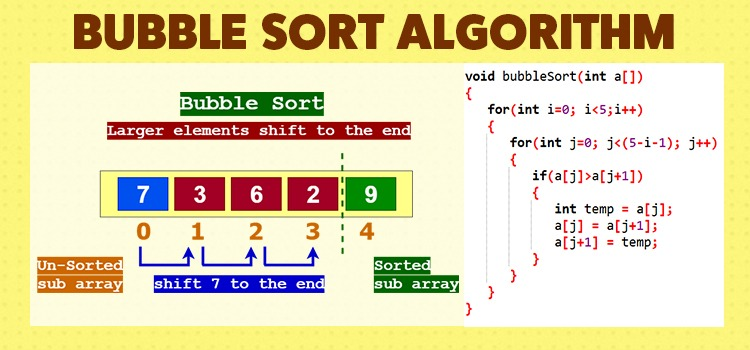
\includegraphics[scale=0.4]{download.jpg}
    \caption{algoritmo\citep{ef}}
    \label{fig:my_label}
\end{figure}

\section{Relêvancia}
Algoritmos e Estruturas de dados são extremamente importantes para a resolução de problemas e desenvolvimento de aplicações. Por isso, é uma cadeira indispensável para alunos do curso de ciência da computação. Estudamos algoritmos e estruturas de dados para que possamos aprender a escrever programas mais eficientes.\citep{cin}

\section{Relação com outras disciplinas} 
Esta diretamente ligada com a cadeira de Introdução a programação, onde somos introduzidos aos conceitos básicos de algoritmos e estruturas de dados.
 

\bibliographystyle{plain}
\bibliography{reference}

\end{document}
